\section{Metodi e Modelli}

L'approccio utilizzato in questa ricerca si è basato sulla modellazione 
del problema nell'ambito di una rete sociale. L'obiettivo è quello di 
studiare la diffusione di una pandemia virale in un ambiente reale, 
composto principalmente da punti di interesse (PdI) collegati tra loro 
tramite una rete di collegamenti, che assume la forma di un grafo. 

\begin{figure}[!hb]
	\centering
	\begin{subfigure}[b]{0.3\textwidth}
		\centering
		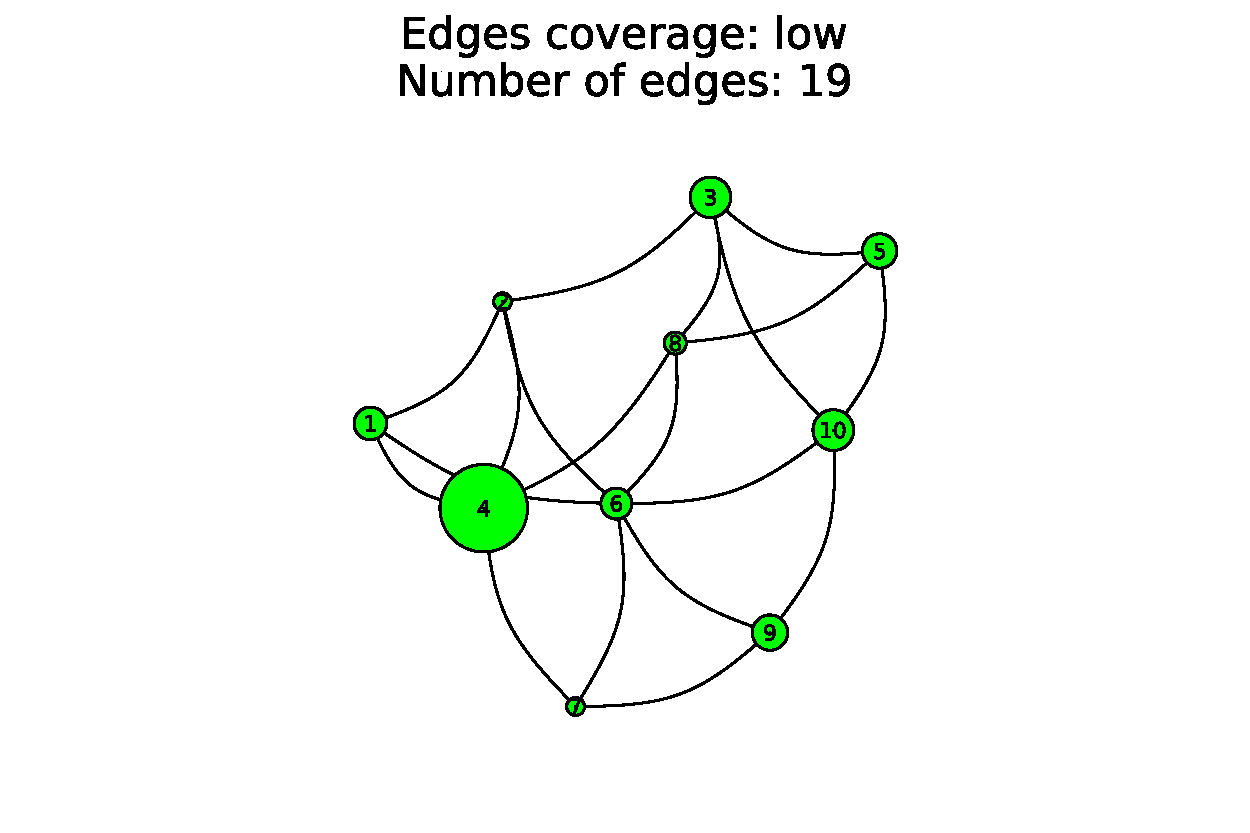
\includegraphics[width=\textwidth]{img/low.pdf}
		\caption{Esempio di grafo connesso con copertura bassa}
		\label{fig:connected_graph_example_low}
	\end{subfigure}
	\hfill
	\begin{subfigure}[b]{0.3\textwidth}
		\centering
		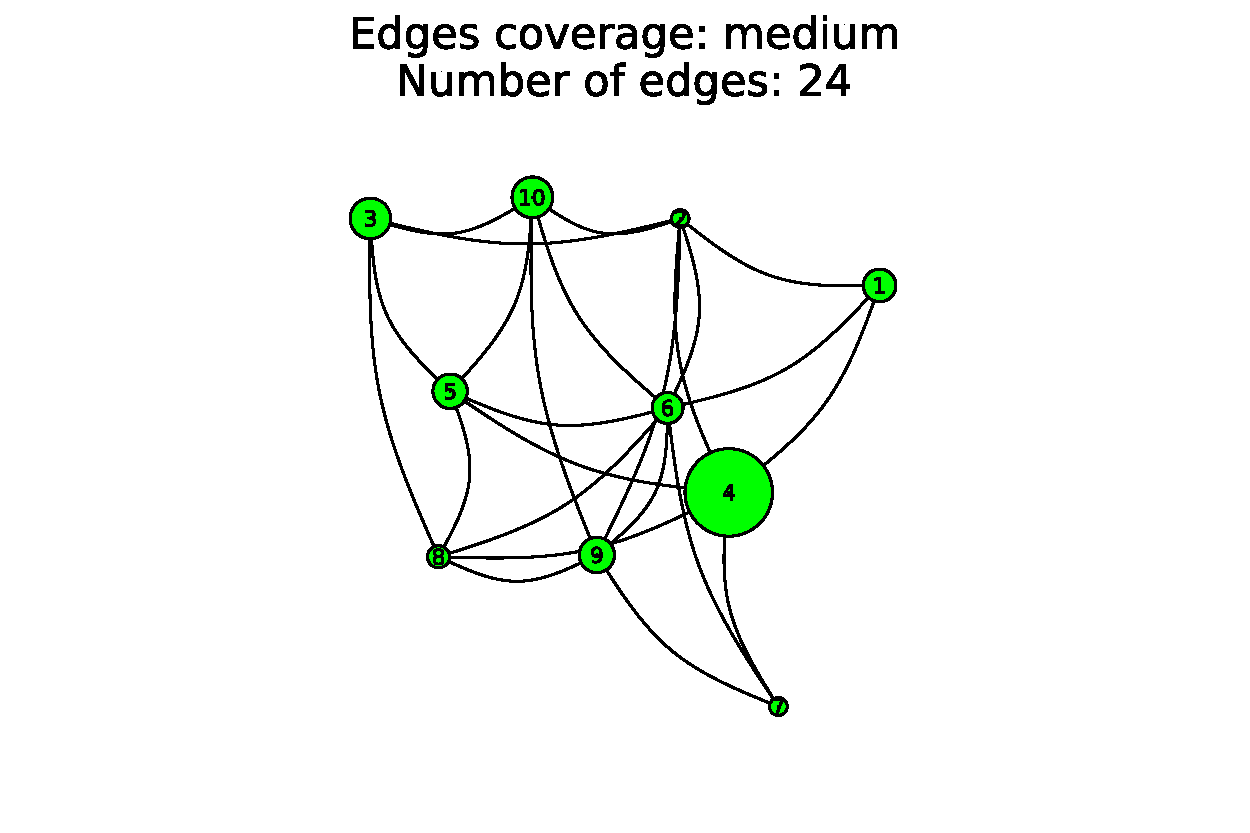
\includegraphics[width=\textwidth]{img/medium.pdf}
		\caption{Esempio di grafo connesso con copertura media}
		\label{fig:connected_graph_example_medium}
	\end{subfigure}
	\hfill
	\begin{subfigure}[b]{0.3\textwidth}
		\centering
		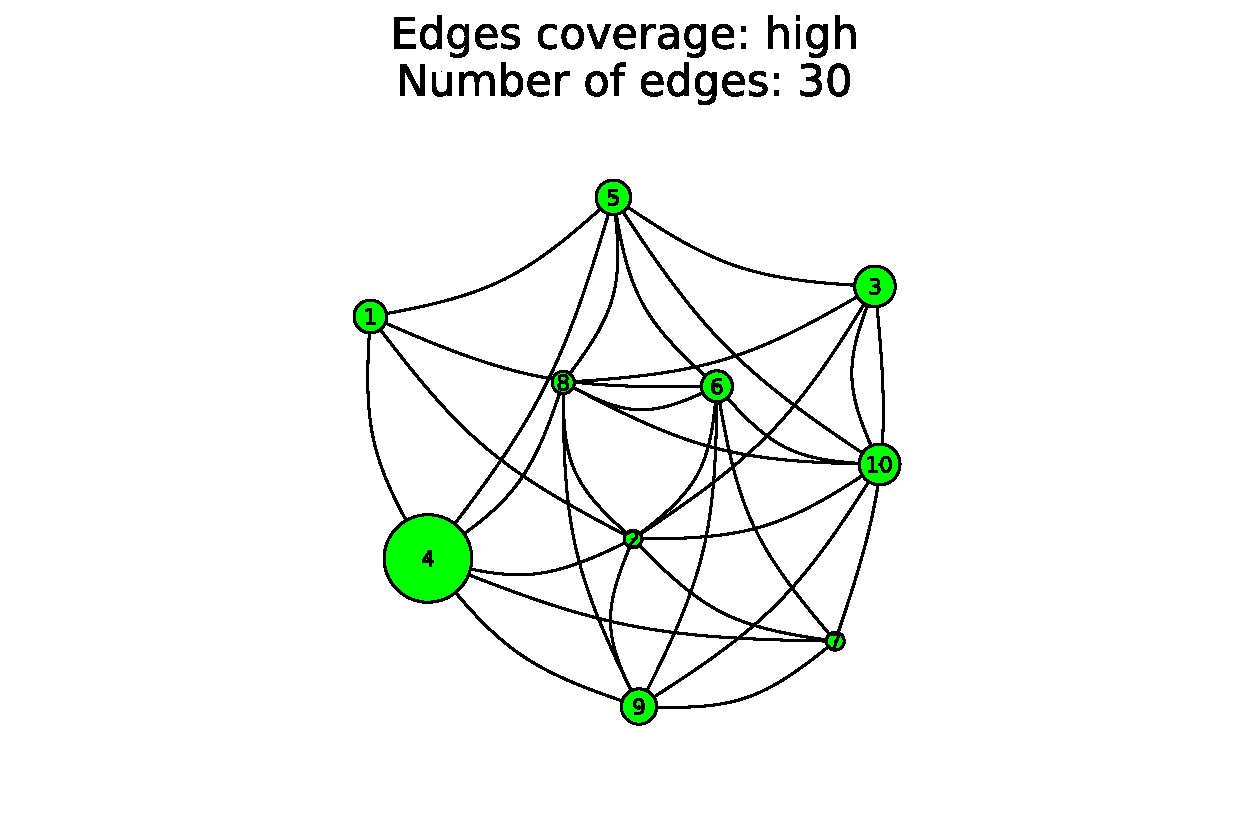
\includegraphics[width=\textwidth]{img/high.pdf}
		\caption{Esempio di grafo connesso con copertura alta}
		\label{fig:connected_graph_example_high}
	\end{subfigure}
\end{figure}

Questo approccio si avvicina a una prospettiva di tipo mesoscopico, 
orientata al macroscopico. La scelta di tale approccio deriva dalla 
necessità di modellare il sistema in maniera più ampia, concentrandosi 
sulla risposta collettiva di un agente astratto agli interventi mirati 
per contrastare l'epidemia in modo localizzato.

\subsection{Approccio con Rete Sociale}

Il modello sviluppato fa uso del framework "Agents.jl" \cite{Agents.jl} e 
definisce un modello ad agenti (ABM). In questo contesto, la struttura 
spaziale del modello non è rilevante, ma le connessioni tra gli agenti 
lo sono. Gli agenti vengono considerati come nodi all'interno di un grafo, 
in cui viene simulato il ciclo di vita della pandemia attraverso un 
modello SEIR deterministico. Gli agenti sono definiti come oggetti di tipo 
"ContinuousAgent", poiché lo spazio del modello è considerato continuo.

La struttura dell'agente è essenziale e include i seguenti campi principali:

\begin{itemize}
	\item \textbf{population}: un intero che rappresenta il numero totale 
	di individui presenti nel nodo.
	\item \textbf{status}: un vettore di numeri decimali che 
	rappresenta lo stato della popolazione nel nodo, espressa 
	come percentuale di individui.
	\item \textbf{param}: un vettore di numeri decimali che contiene 
	i parametri specifici del modello SEIR per il nodo.
	\item \textbf{happiness}: un campo di supporto per il bilanciamento 
	delle contromisure applicate dal controllore.
\end{itemize}

\subsubsection{Grafo Sociale}

Un grafo sociale è un tipo di grafo che rappresenta le relazioni sociali 
tra le entità. In questo contesto, i nodi del grafo rappresentano gli 
individui e gli archi rappresentano le loro relazioni sociali. 
Questo approccio è spesso utilizzato per modellare le reti sociali, 
dove gli individui sono i nodi e le loro connessioni sono gli archi.

\begin{minipage}{\linewidth}
    \centering
    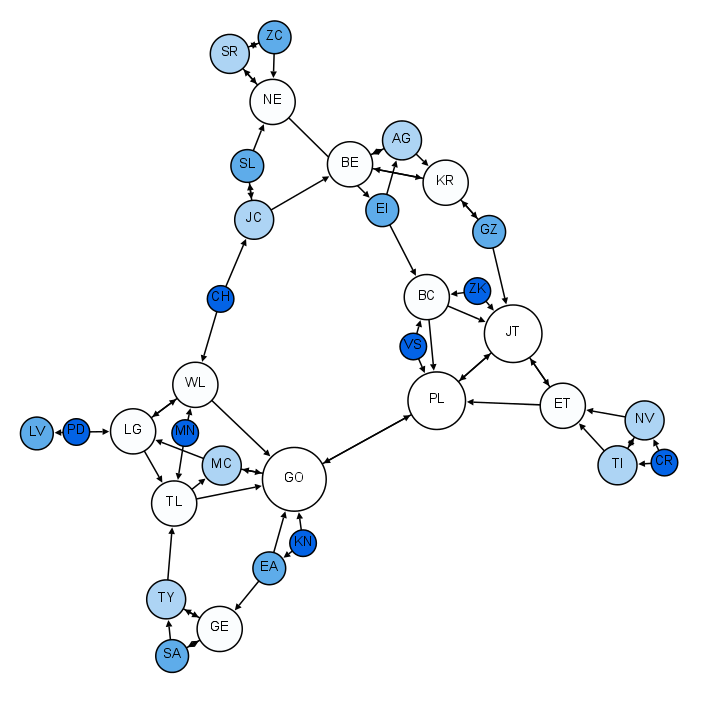
\includegraphics[width=\textwidth]{img/Moreno_Sociogram_3rd_Grade.png}
    \captionof{figure}{Moreno's Sociagram of a 3rd grade class}
	\url{https://en.wikipedia.org/wiki/Sociogram#/media/File:Moreno_Sociogram_3rd_Grade.png}
    \label{fig:social_graph}
\end{minipage}

\subsection{Agente}

L'agente è stato implementato in modo minimale e contiene solo gli 
attributi essenziali per il funzionamento del modello e le 
interazioni con l'ambiente e gli altri agenti. L'evoluzione di ogni 
agente è indipendente dagli altri, ma può essere influenzata da agenti 
nella stessa rete.

\begin{minipage}{\linewidth}
    \centering
    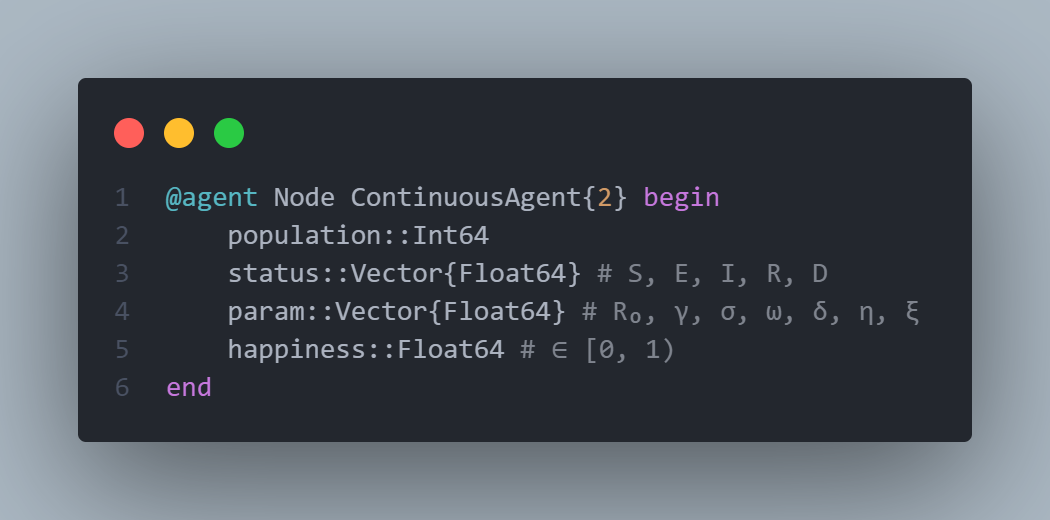
\includegraphics[width=\textwidth]{img/node_agent.png}
    \captionof{figure}{Codice Agente}
    \label{fig:Agent_code}
\end{minipage}

\subsection{Spazio e Modello}

\begin{minipage}{\linewidth}
    \centering
    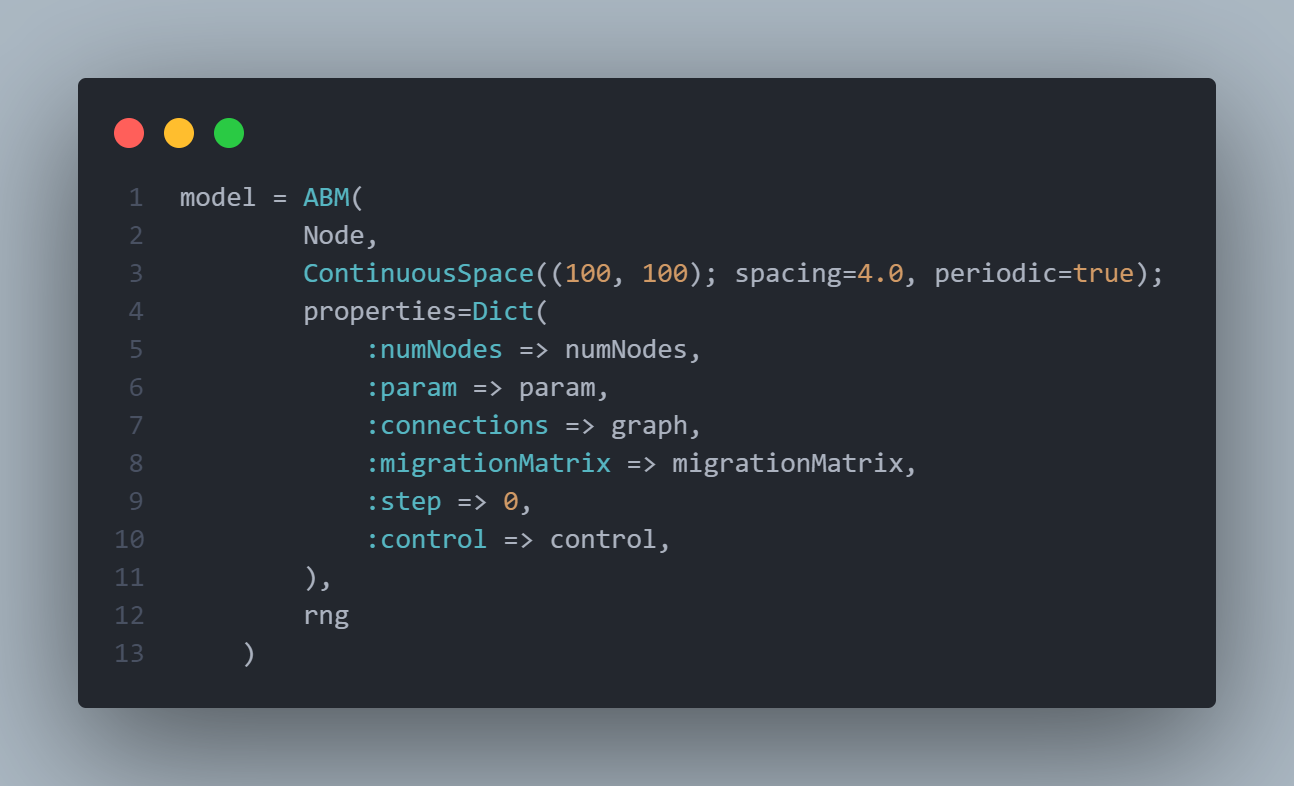
\includegraphics[width=\textwidth]{img/sngraph_model.png}
    \captionof{figure}{Codice Modello}
    \label{fig:Model_code}
\end{minipage}

Lo spazio del modello è basato su un grafo connesso, dove il numero 
di archi dipende dalla copertura desiderata degli archi. La topologia 
del grafo è creata in base alle preferenze dell'utente, con un limite 
inferiore dato dalla connessione minima e un limite superiore dato 
dalla connessione completa.

\begin{figure}[!hb]
	\centering
	\begin{subfigure}[b]{0.45\textwidth}
		\centering
		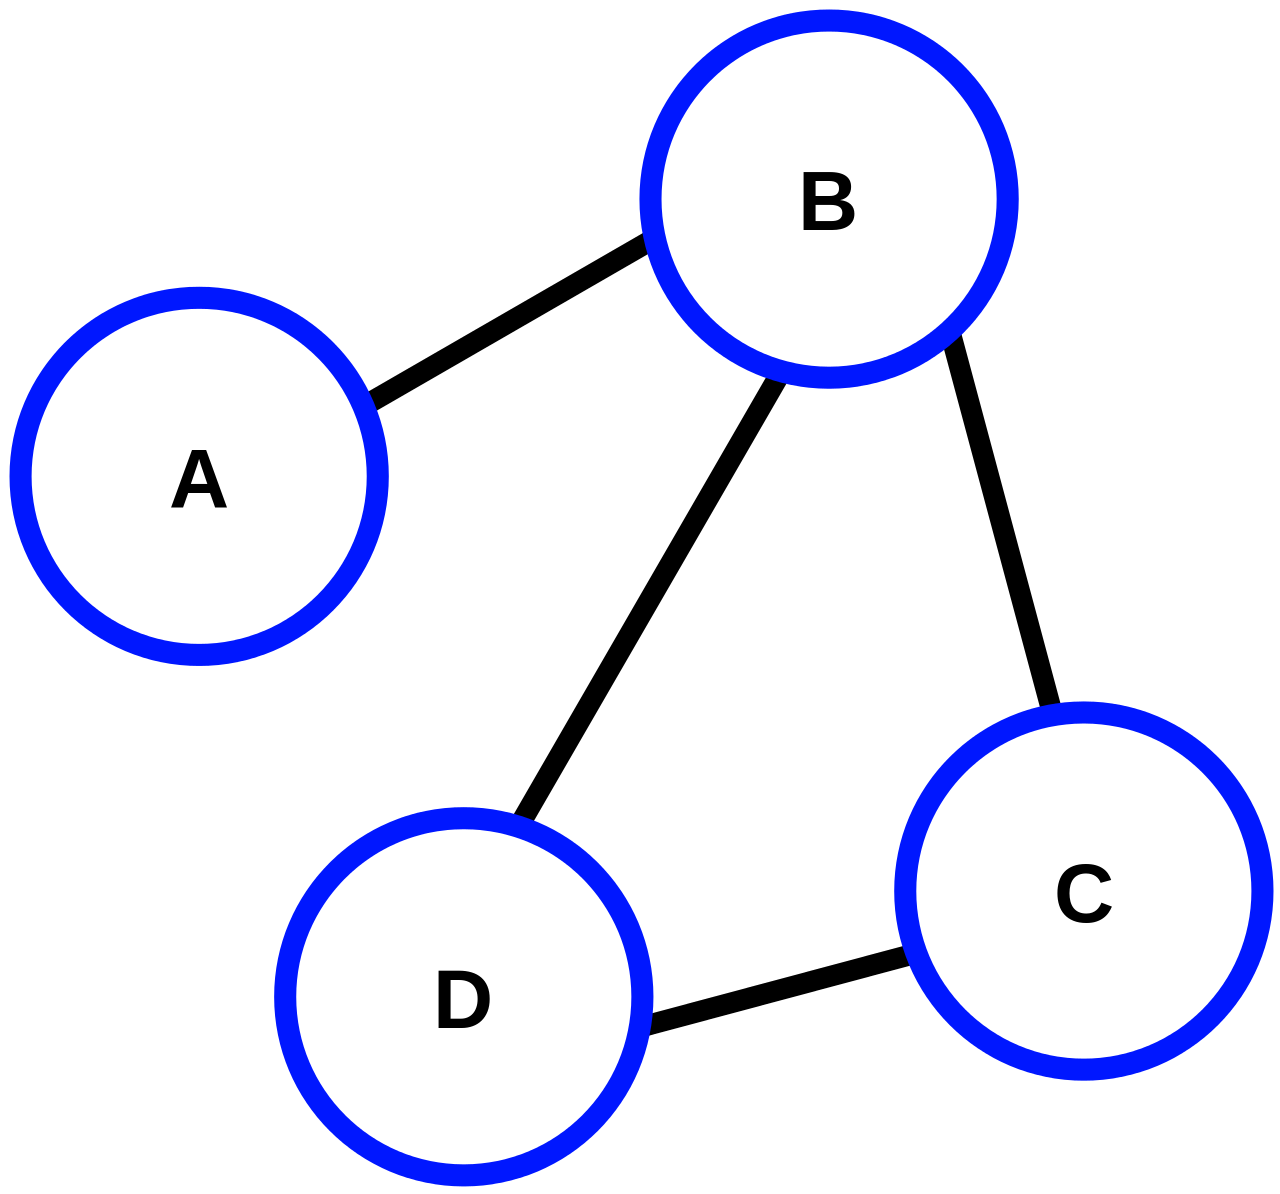
\includegraphics[width=\textwidth]{img/CPT-Graphs-undirected-unweighted-ex1.svg.png}
		\caption{Esempio di grafo connesso}
		\url{https://it.wikipedia.org/wiki/Grafo_connesso#/media/File:CPT-Graphs-undirected-unweighted-ex1.svg}
		\label{fig:connected_graph_example}
	\end{subfigure}
	\hfill
	\begin{subfigure}[b]{0.45\textwidth}
		\centering
		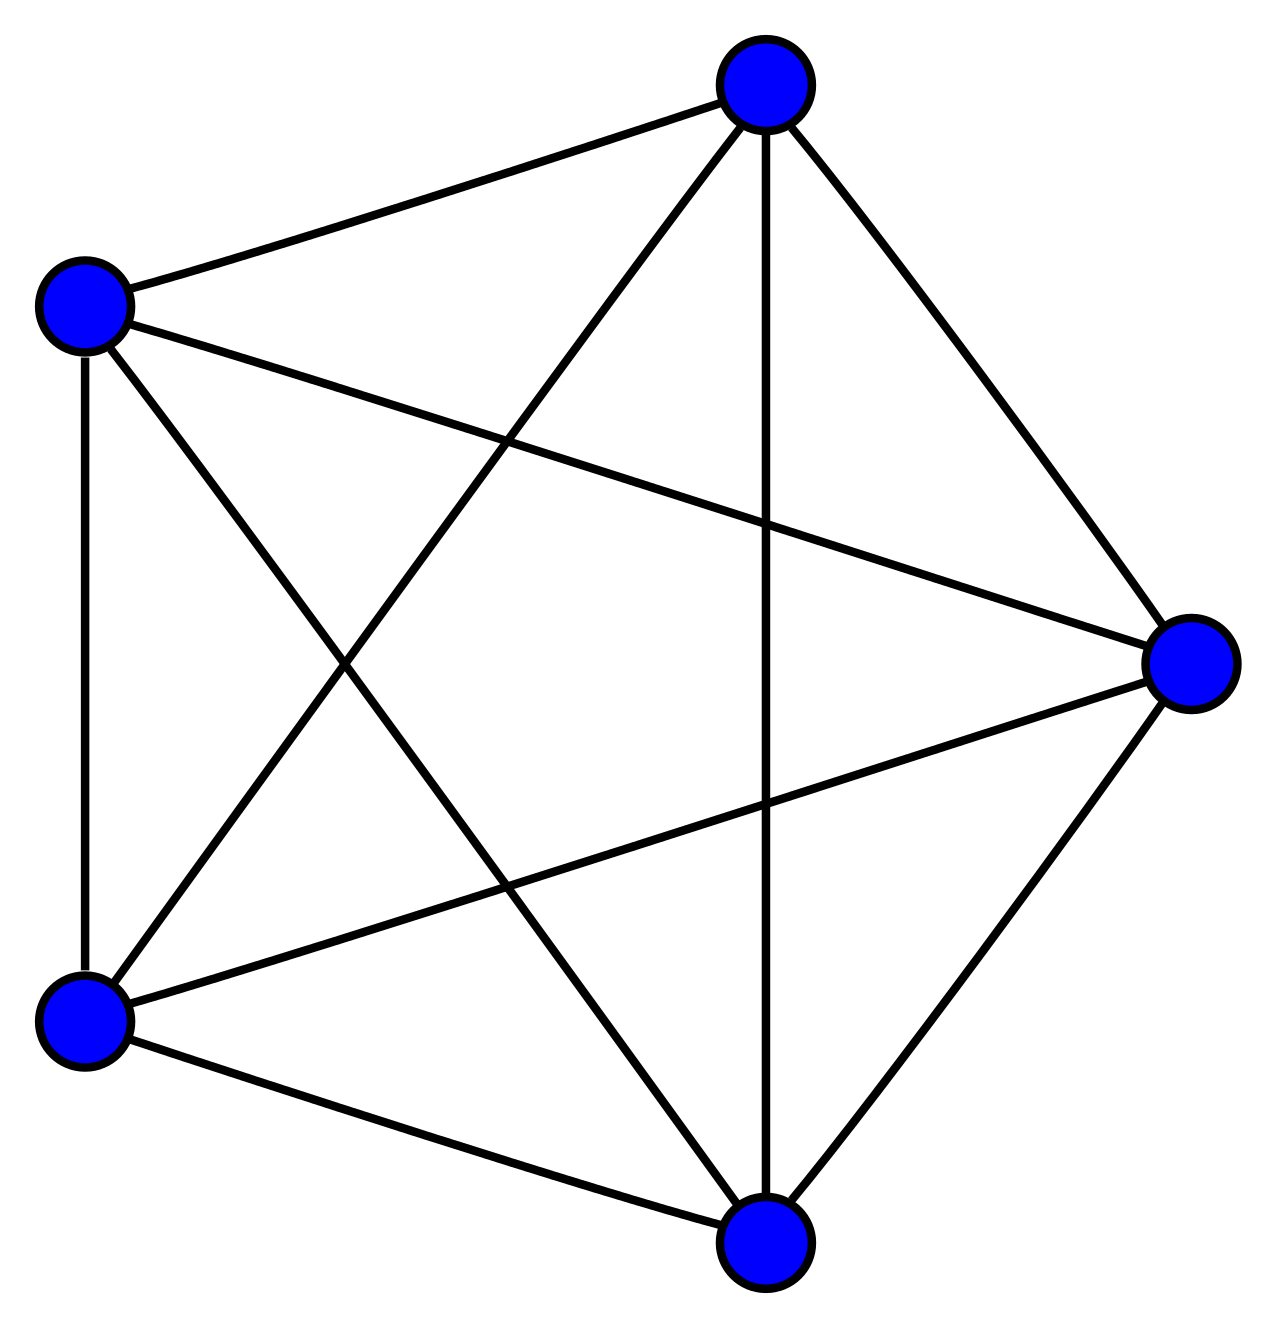
\includegraphics[width=\textwidth]{img/4-simplex_graph.svg.png}
		\caption{Esempio di grafo completo}
		\url{https://en.wikipedia.org/wiki/Complete_graph#/media/File:4-simplex_graph.svg}
		\label{fig:complete_graph_example}
	\end{subfigure}
\end{figure}

\subsection{Funzione di Avanzamento Agente}

Ogni agente segue un ciclo di comportamento che include tre compiti 
principali: spostarsi tra i nodi del grafo \cite{Ding2021}, calcolare 
il proprio "livello di felicità" e chiamare il controllore per 
valutare le misure di intervento necessarie.

\begin{minipage}{\linewidth}
	\centering
	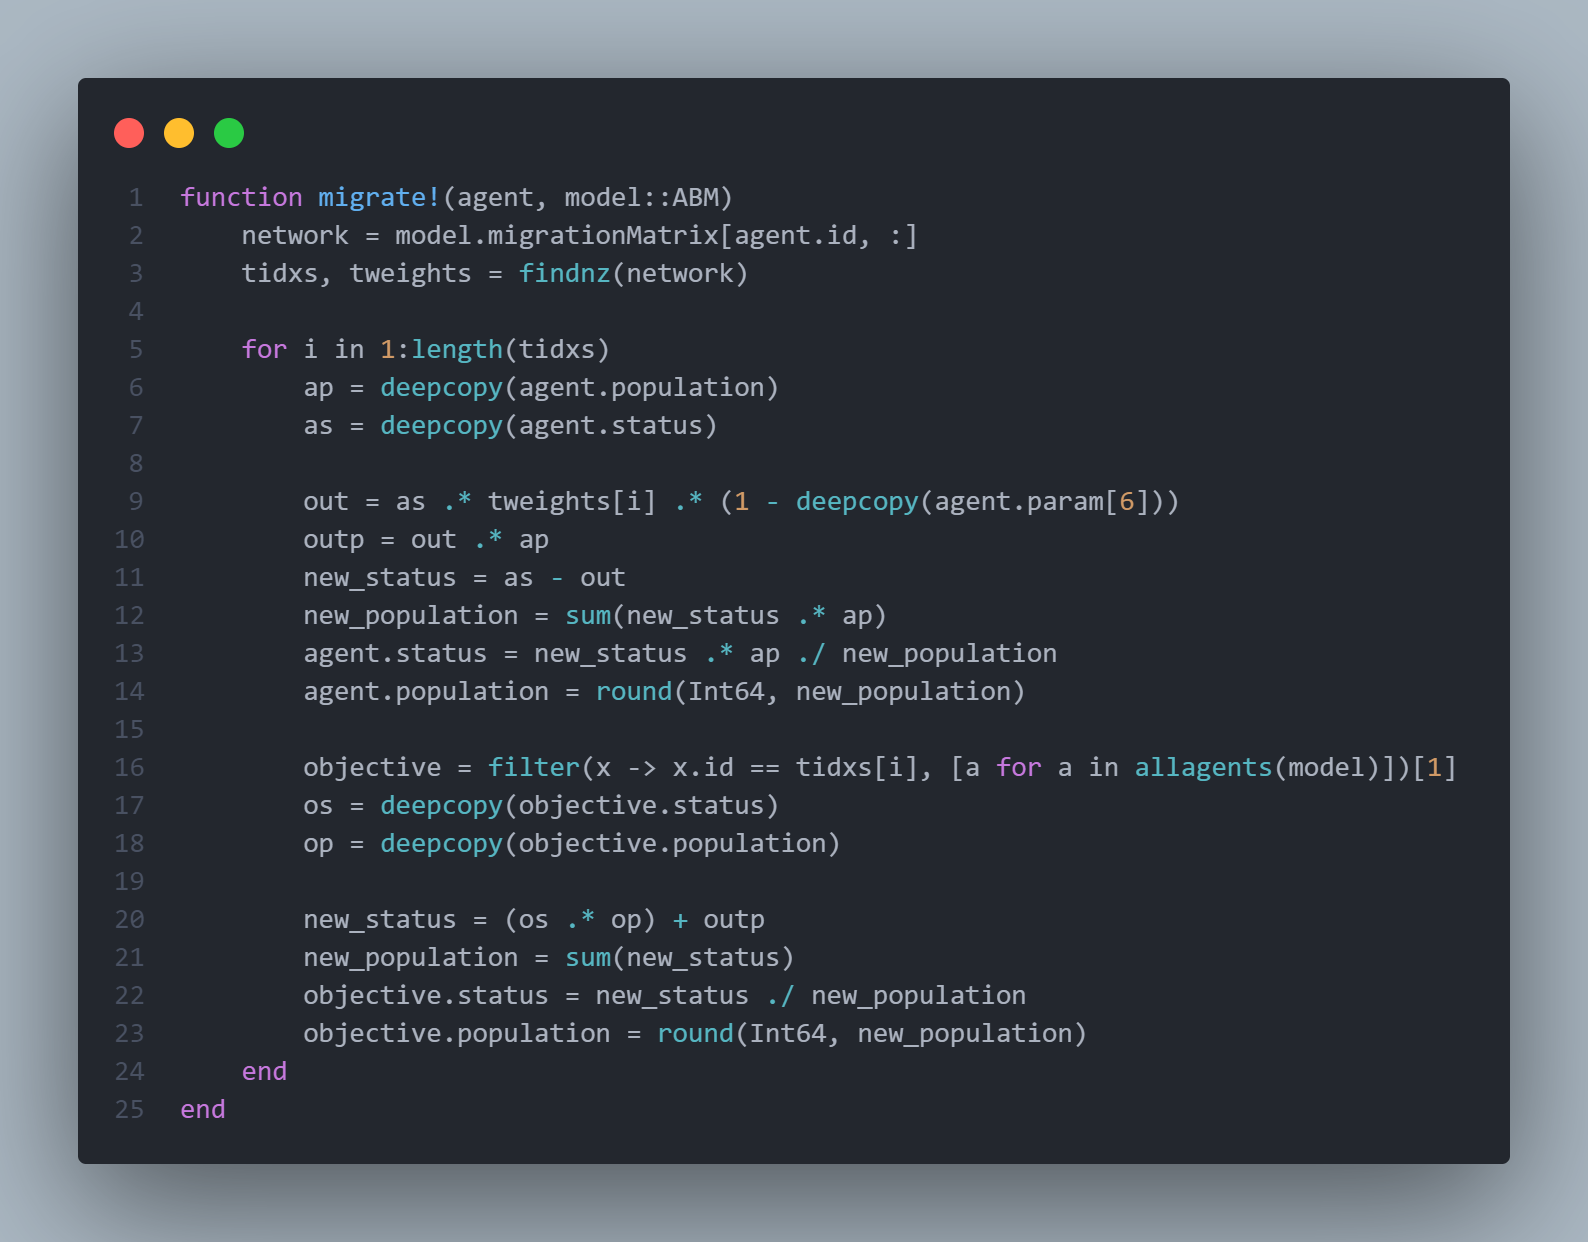
\includegraphics[width=\textwidth]{img/migratef.png}
	\captionof{figure}{Funzione atta a calcolare lo spostamento di agenti da un nodo all'altro del grafo}
	\label{fig:migrationf}
\end{minipage}

\begin{minipage}{\linewidth}
	\centering
	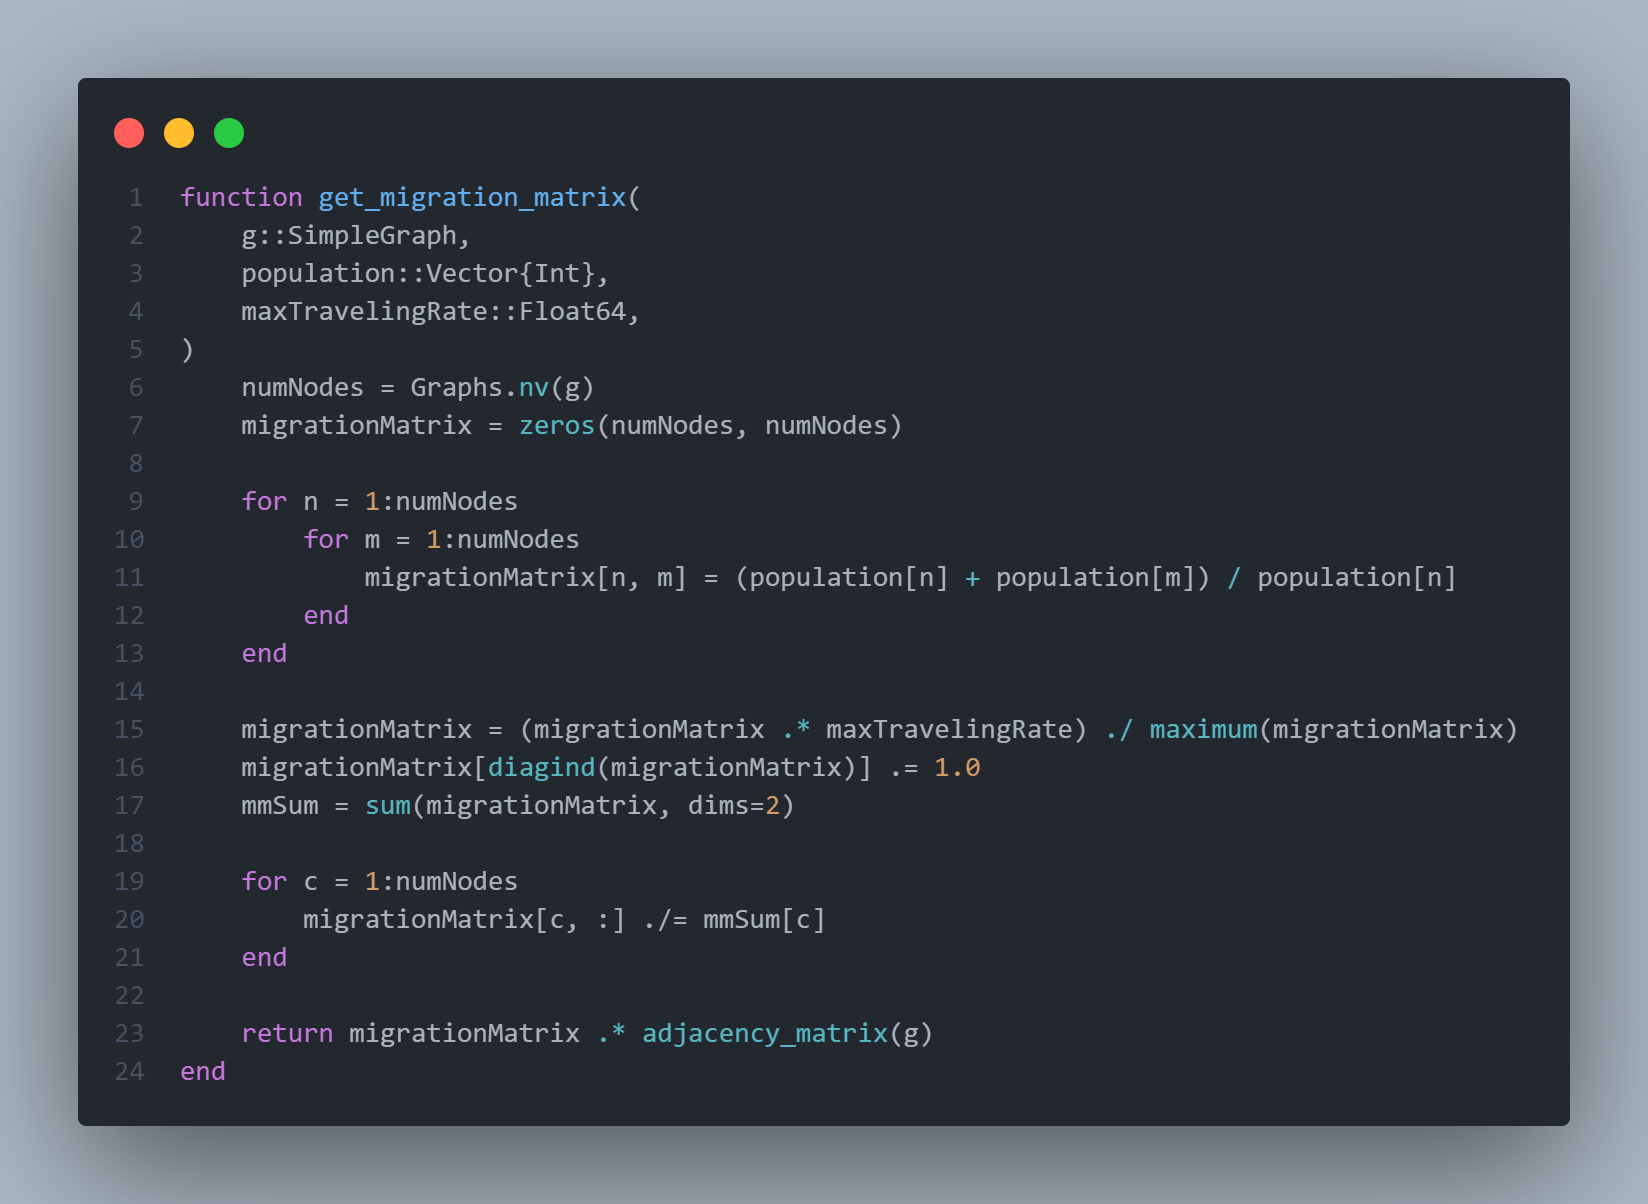
\includegraphics[width=\textwidth]{img/mmfunc.png}
	\captionof{figure}{Funzione che crea la matrice di migrazione data la topologia di un grafo}
	\label{fig:migration_matrix_function}
\end{minipage}

\begin{minipage}{\linewidth}
	\centering
	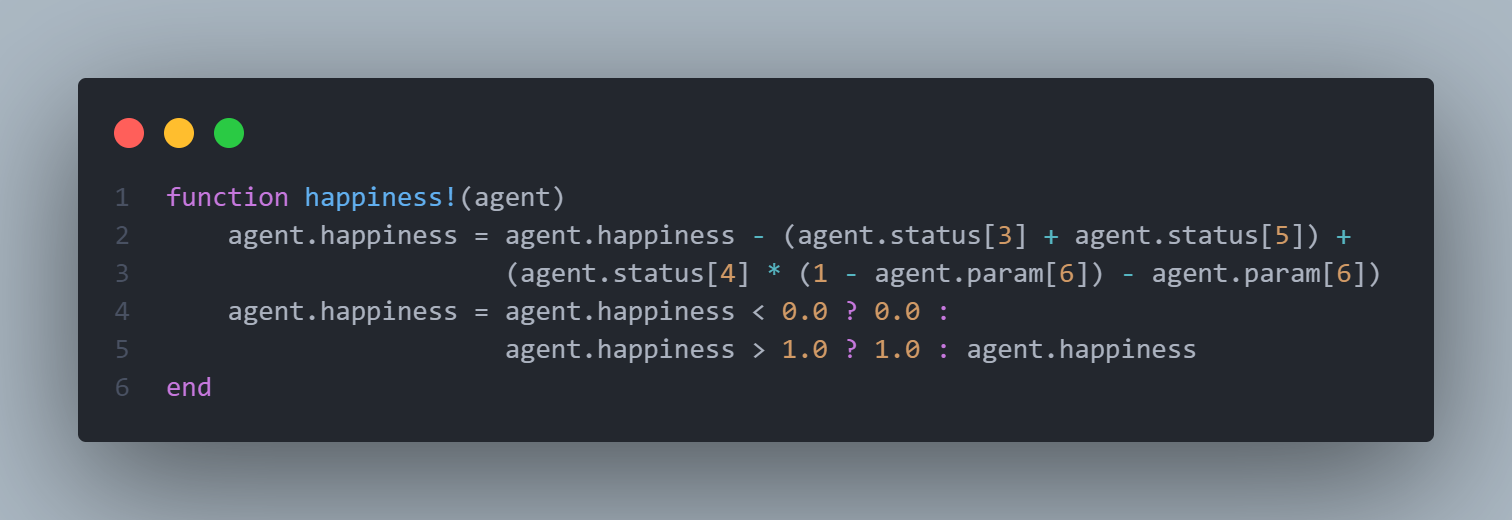
\includegraphics[width=\textwidth]{img/happiness.png}
	\captionof{figure}{Funzione atta a calcolare la felicità degli agenti}
	\label{fig:happinessf}
\end{minipage}

\subsection{Funzione di Avanzamento Modello}

Il modello coordina l'avanzamento degli agenti e si occupa di 
operazioni che coinvolgono l'intero sistema invece di singoli agenti. 
Queste operazioni includono l'aggiornamento delle equazioni 
differenziali ordinarie (ODE) associate a ciascun agente e la gestione 
delle varianti del virus di interesse.

\subsubsection{Funzione per la Generazione delle Varianti del Virus (VOC)}

La generazione delle VOC è basata su alcune assunzioni, tra cui un 
tasso di mutazione casuale delle basi del virus e una distribuzione 
dei parametri pandemici. Questa semplice implementazione rappresenta 
un'approssimazione del comportamento delle varianti. \cite{Markov2023} 
\cite{https://doi.org/10.1002/jmv.27331} \cite{Abavisani2022}

\begin{minipage}{\linewidth}
	\centering
	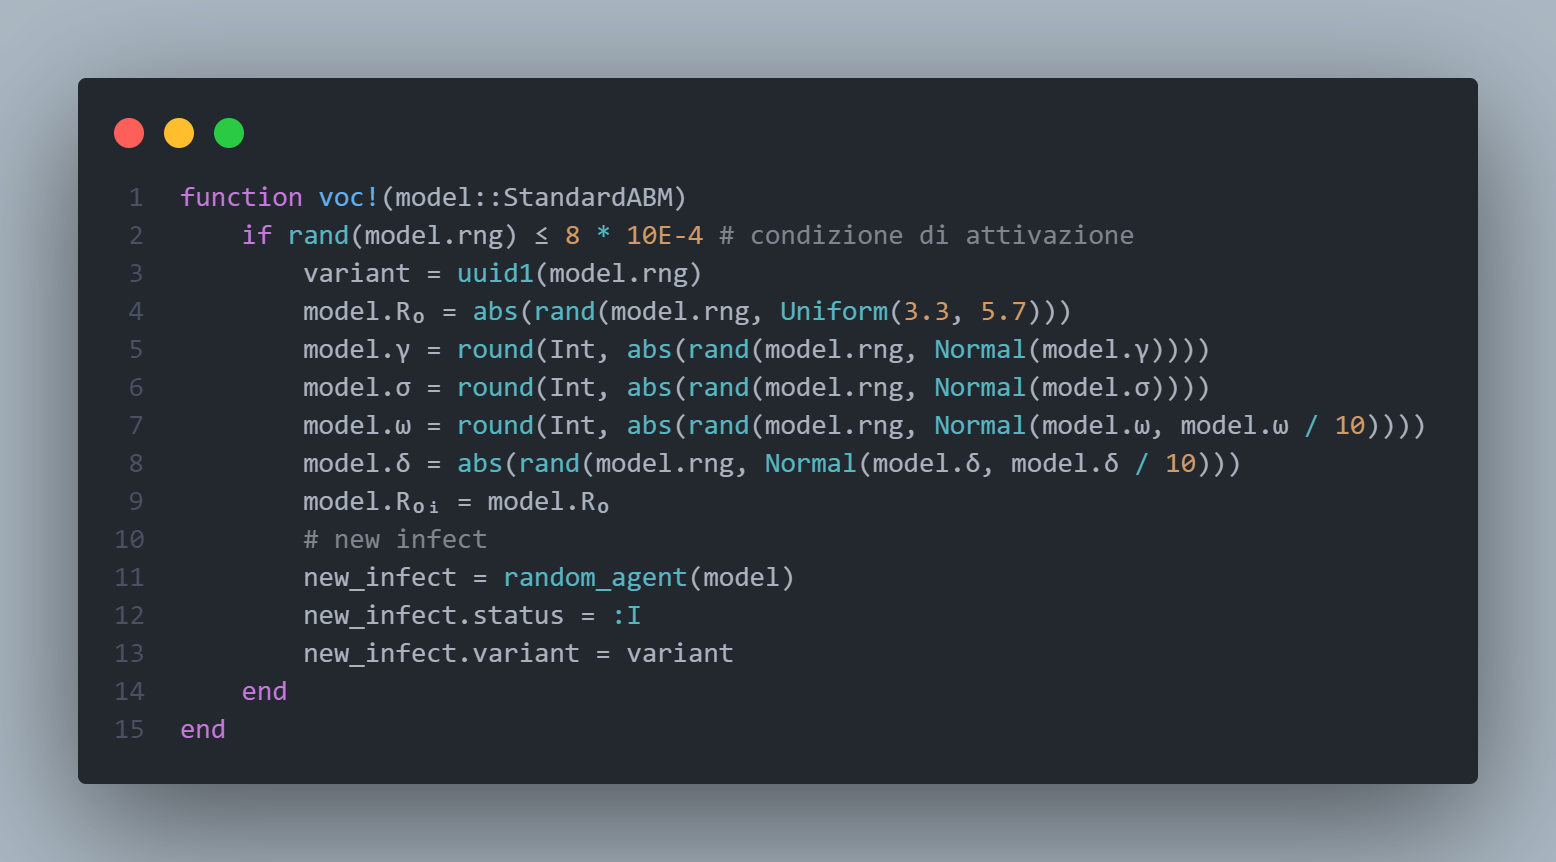
\includegraphics[width=\textwidth]{img/voc.png}
	\captionof{figure}{Funzione che si occupa di generare la VOC}
	\label{fig:voc}
\end{minipage}

\subsubsection{Funzione per la Simulazione della Campagna di Vaccinazione}

La simulazione della campagna di vaccinazione si basa su una 
percentuale fissa di popolazione vaccinata a ciascun passo del modello. 
Questa percentuale tiene conto dell'immunità di gregge da raggiungere 
entro un periodo specifico.

\begin{minipage}{\linewidth}
	\centering
	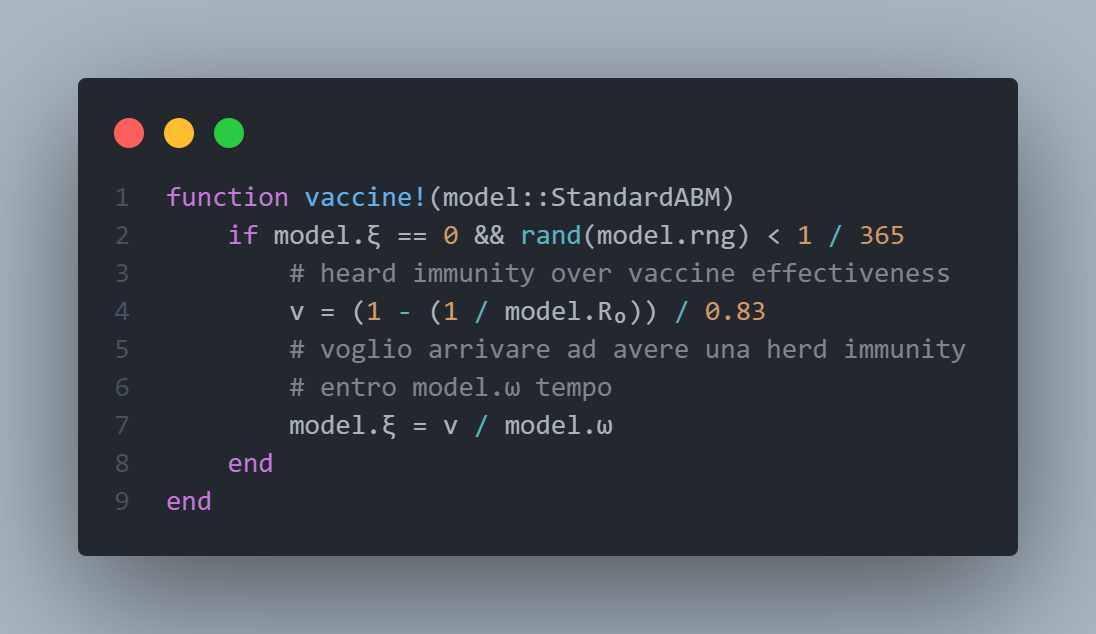
\includegraphics[width=\textwidth]{img/vaccine.png}
	\captionof{figure}{Funzione che si occupa di simulare la ricerca di un vaccino e la sua successiva applicazoine}
	\label{fig:vaccine}
\end{minipage}

Queste funzioni sono soggette a diverse assunzioni, tra cui l'effetto 
delle mutazioni del virus sulla distribuzione dei parametri pandemici e 
il meccanismo di vaccinazione basato su dosi fisse. Le assunzioni 
semplificano il modello, ma possono non rappresentare completamente 
il comportamento del mondo reale.

\subsubsection*{Grafici di Confronto}

I grafici di confronto mostrano l'impatto del momento di inizio della 
campagna di vaccinazione su diversi scenari. Questi grafici illustrano 
come l'efficacia della campagna vaccinale possa dipendere dal suo avvio, 
oltre al numero di persone vaccinate.

\begin{figure}[!hb]
	\centering
	\begin{subfigure}[b]{0.45\textwidth}
		\centering
		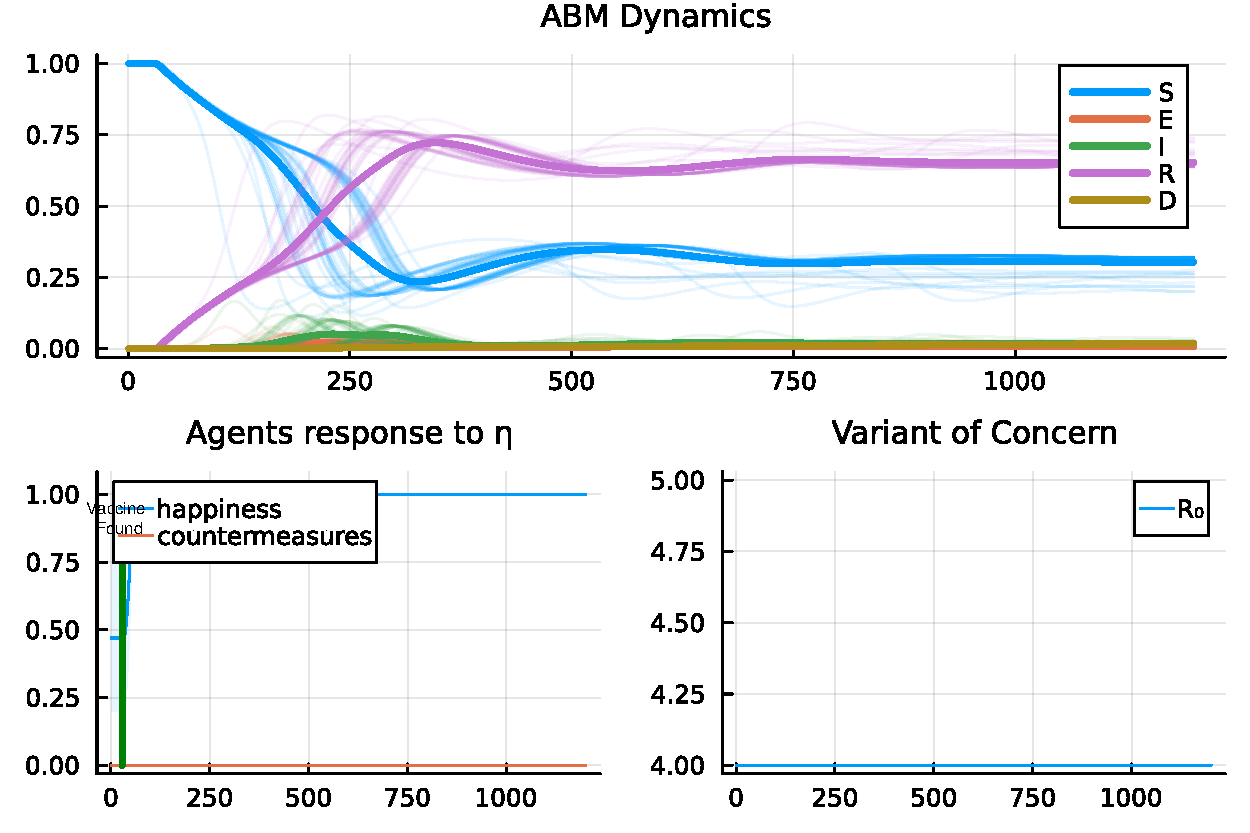
\includegraphics[width=\textwidth]{img/SocialNetworkABM_4_V.pdf}
		\caption{Grafico per la comparazione sul periodo di inizio della campagna vaccinale. Immediata}
		\label{fig:comparison_vax_1}
	\end{subfigure}
	\hfill
	\begin{subfigure}[b]{0.45\textwidth}
		\centering
		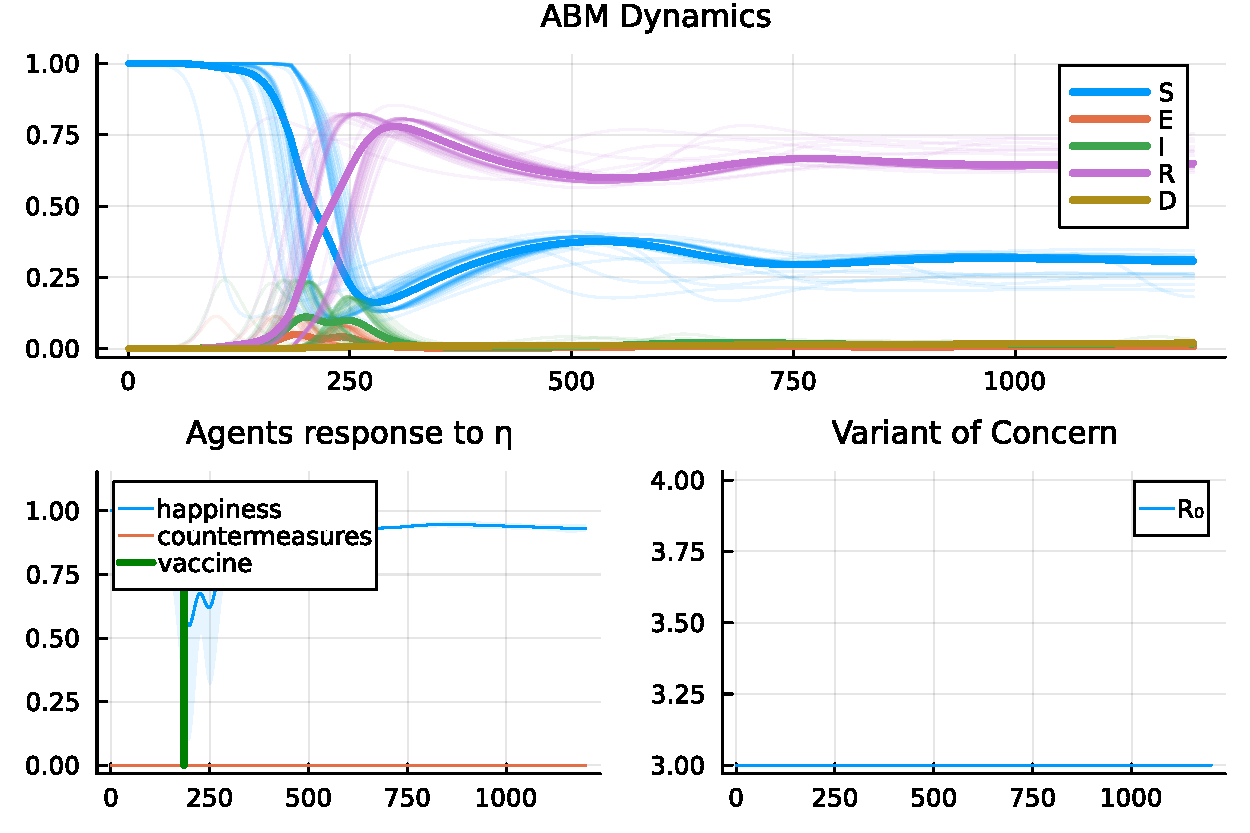
\includegraphics[width=\textwidth]{img/SocialNetworkABM_3_V.pdf}
		\caption{Grafico per la comparazione sul periodo di inizio della campagna vaccinale. Durante prima ondata}
		\label{fig:comparison_vax_2}
	\end{subfigure}
	\hfill
	\begin{subfigure}[b]{0.45\textwidth}
		\centering
		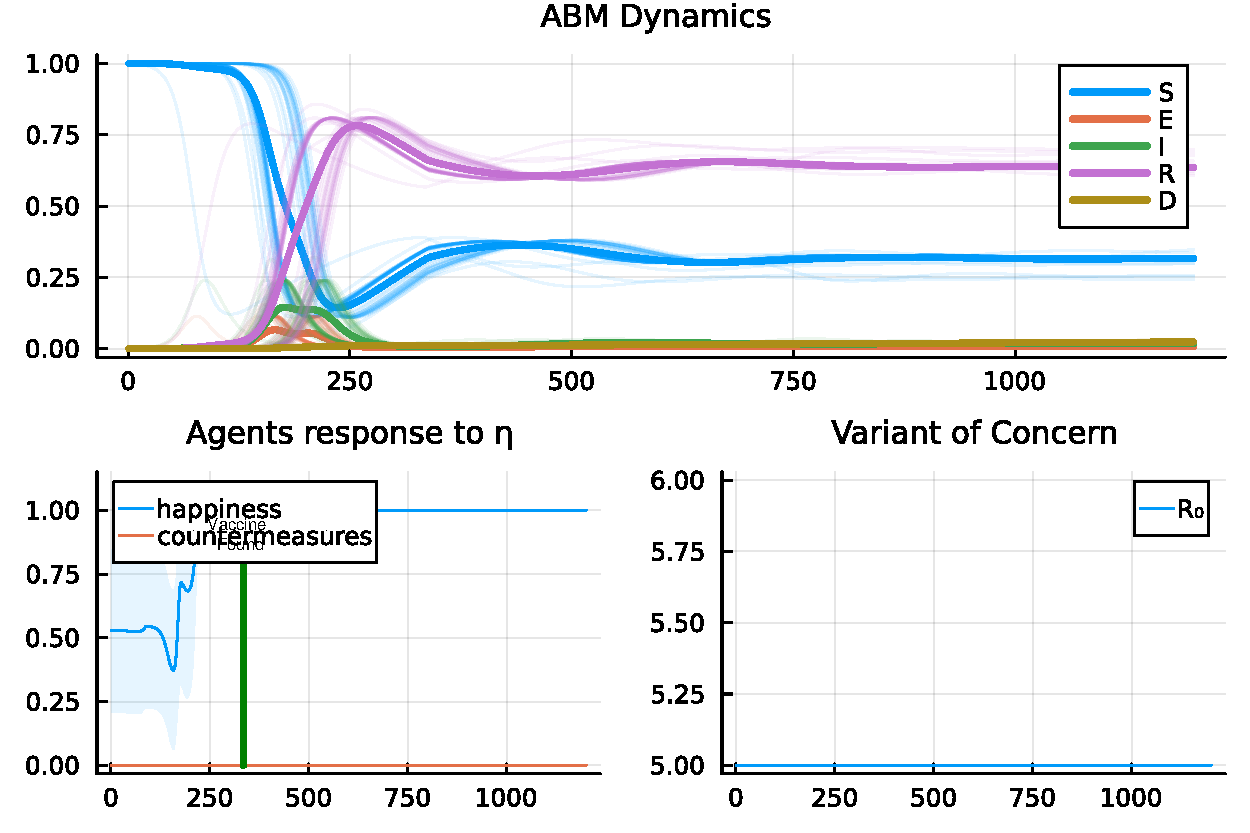
\includegraphics[width=\textwidth]{img/SocialNetworkABM_5_V.pdf}
		\caption{Grafico per la comparazione sul periodo di inizio della campagna vaccinale. Poco dopo la prima ondata}
		\label{fig:comparison_vax_3}
	\end{subfigure}
	\hfill
	\begin{subfigure}[b]{0.45\textwidth}
		\centering
		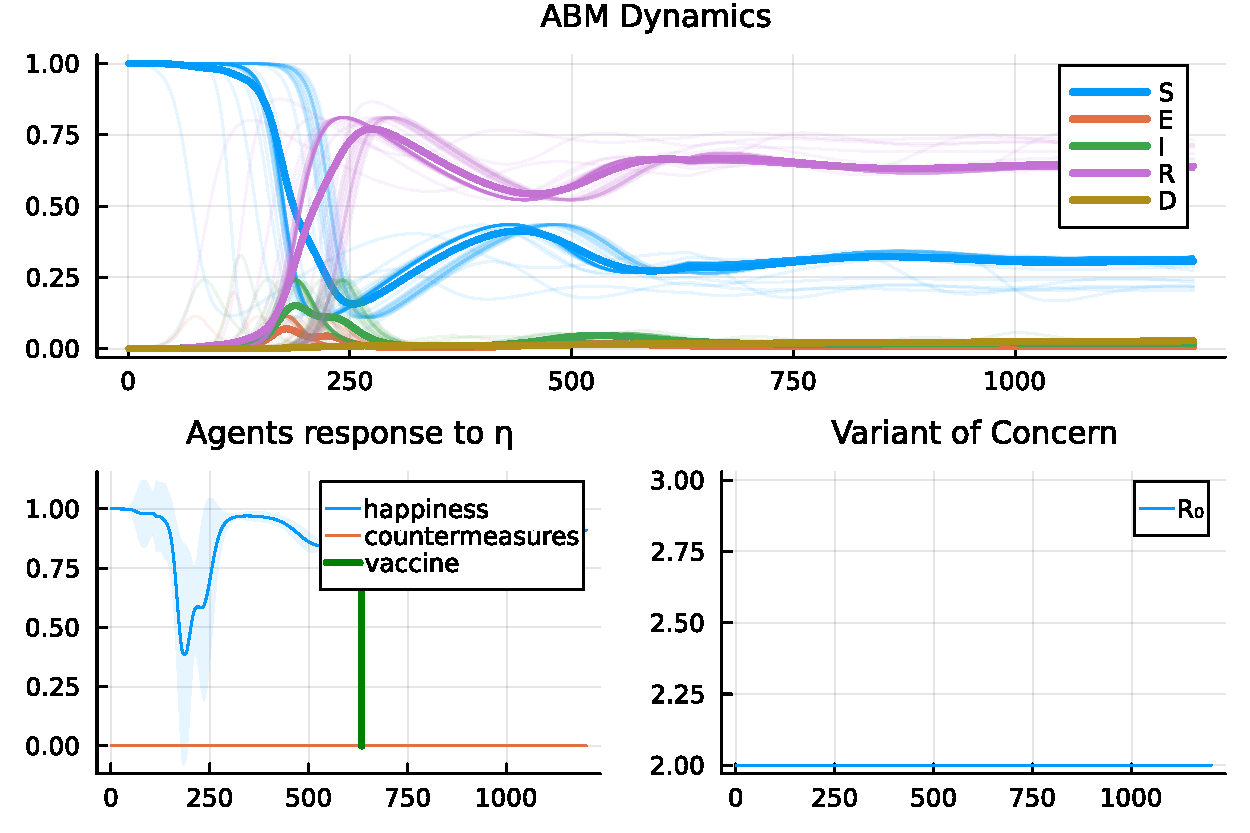
\includegraphics[width=\textwidth]{img/SocialNetworkABM_2_V.pdf}
		\caption{Grafico per la comparazione sul periodo di inizio della campagna vaccinale. In ritardo}
		\label{fig:comparison_vax_4}
	\end{subfigure}
\end{figure}